\documentclass[aspectratio=169,11pt]{beamer}
\usetheme{default}
\usecolortheme{default}
\setbeamertemplate{navigation symbols}{}
\setbeamertemplate{footline}[frame number]
\setbeamercolor{frametitle}{fg=black!85}
\setbeamercolor{structure}{fg=blue!55!black}
\usepackage{booktabs}
\usepackage{graphicx}
\graphicspath{{../01_reporte/figures/}}
\newcommand{\deltaMain}{$-$0.013}
\newcommand{\ciMain}{[$-$0.027, +0.002]}
\newcommand{\resBetter}{7 of 24}
\newcommand{\eegBetter}{17}
\newcommand{\resMainSubj}{0.761}
\newcommand{\eegMainSubj}{0.774}
\newcommand{\hypVerdict}{not supported}
\newcommand{\mainVerdict}{the interval includes zero, so the CNN on scalograms is not better than EEGNet on the raw signal; the two are statistically indistinguishable.}
\newcommand{\deltaInitial}{$-$0.005}
\newcommand{\deltaOldLr}{$-$0.024}
\newcommand{\ciOldLr}{[$-$0.037, $-$0.009]}
\newcommand{\oldLrSubj}{0.750}
\newcommand{\oldLrBetter}{5 of 24}
\newcommand{\deltaLrGain}{+0.011}
\newcommand{\ciLrGain}{[+0.005, +0.017]}
\newcommand{\lrGainBetter}{18 of 24}
\newcommand{\deltaCuda}{$-$0.007}
\newcommand{\ciCuda}{[$-$0.023, +0.009]}
\newcommand{\deltaCudaMps}{+0.006}
\newcommand{\ciCudaMps}{[$-$0.002, +0.013]}
\newcommand{\deltaCudaPair}{+0.000}
\newcommand{\ciCudaPair}{[$-$0.015, +0.017]}
\newcommand{\deltaStftCuda}{+0.006}
\newcommand{\ciStftCuda}{[$-$0.000, +0.012]}
\newcommand{\deltaScratch}{+0.015}
\newcommand{\ciScratch}{[+0.004, +0.025]}
\newcommand{\scratchSubj}{0.735}
\newcommand{\deltaStft}{+0.007}
\newcommand{\ciStft}{[$-$0.005, +0.019]}
\newcommand{\stftSubj}{0.755}
\newcommand{\deltaStftOld}{$-$0.001}
\newcommand{\ciStftOld}{[$-$0.010, +0.007]}
\newcommand{\stftVerdict}{indistinguishably}
\newcommand{\stftSentence}{the interval includes zero, so the choice of time--frequency transform does not measurably matter here.}
\newcommand{\stftShort}{makes no measurable difference}
\newcommand{\worstRange}{0.65 to 0.89 for EEGNet}
\newcommand{\worstSubjects}{22 (0.65, 51\% slow), 9 (0.69, 34\% slow), 31 (0.71, 21\% slow), 6 (0.71, 20\% slow)}
\newcommand{\condText}{0.791 (motion) vs.\ 0.782 (motionless) for EEGNet and 0.759 vs.\ 0.760 for ResNet18; a descriptive, not pre-registered, contrast.}
\newcommand{\agreePct}{86.2\%}
\newcommand{\disagree}{EEGNet 58.3\% vs.\ ResNet18 41.7\%}
\newcommand{\bothWrongSlow}{32.2\%}


\title{Images or raw signal?}
\subtitle{Decoding a subject-relative response state from pre-event EEG on unseen subjects}
\author{Juan Pablo Acevedo Robles \& Alberto Martinez Hernandez\\[2pt] Team 8}
\date{Deep Learning -- Final project}

\begin{document}

\begin{frame}
\titlepage
\end{frame}

% ~1 min
\begin{frame}{Thesis context and sub-objective}
\begin{columns}[T]
\column{0.5\textwidth}
\textbf{Alberto:} quantification and standardization of \textbf{pain} from EEG.
\begin{itemize}\small
\item Self-report (0--10) is subjective and not comparable across people.
\item EEG marker $\Rightarrow$ must work on \emph{people the model has not seen}.
\end{itemize}
\textbf{Juan Pablo:} real-time \textbf{trust} in autonomous driving from physiological signals.
\column{0.5\textwidth}
\textbf{Shared question:} which EEG representation generalizes best to new people, for a state defined \emph{relative to each person}?

\medskip
Our datasets ($\geq$40 subjects each) are still being collected, so a public driving dataset is the testbed (indirect link).

\medskip
\textbf{Sub-objective:} predict fast vs.\ slow response from pre-event EEG, and test whether an image representation generalizes better than the raw signal.
\end{columns}
\end{frame}

% ~1 min
\begin{frame}{Problem formulation and hypothesis}
\begin{itemize}
\item \textbf{Input:} 3\,s before lane deviation, Fz/Pz/Oz, 1--50\,Hz, 250\,Hz $\rightarrow 3\times750$
\item \textbf{Output:} $p(\text{slow})$. Label from reaction time relative to the session's 5th percentile: fast $<1.5\times$, slow $>2.5\times$
\item \textbf{Task:} supervised binary classification, tested on \textbf{unseen subjects}
\end{itemize}
\begin{block}{Hypothesis (falsifiable)}
ResNet18 (ImageNet) on wavelet scalograms reaches higher balanced accuracy on unseen subjects than EEGNet on the raw signal, with the same data, folds, seeds, loss, early stopping and tuning budget.
\end{block}
\textbf{Decision rule:} $\Delta$ = BA(ResNet18) $-$ BA(EEGNet) per subject; supported if mean $\Delta>0$ \emph{and} the 95\% subject-bootstrap CI excludes 0.
\end{frame}

% ~2 min
\begin{frame}{Data, method and baselines}
\centering
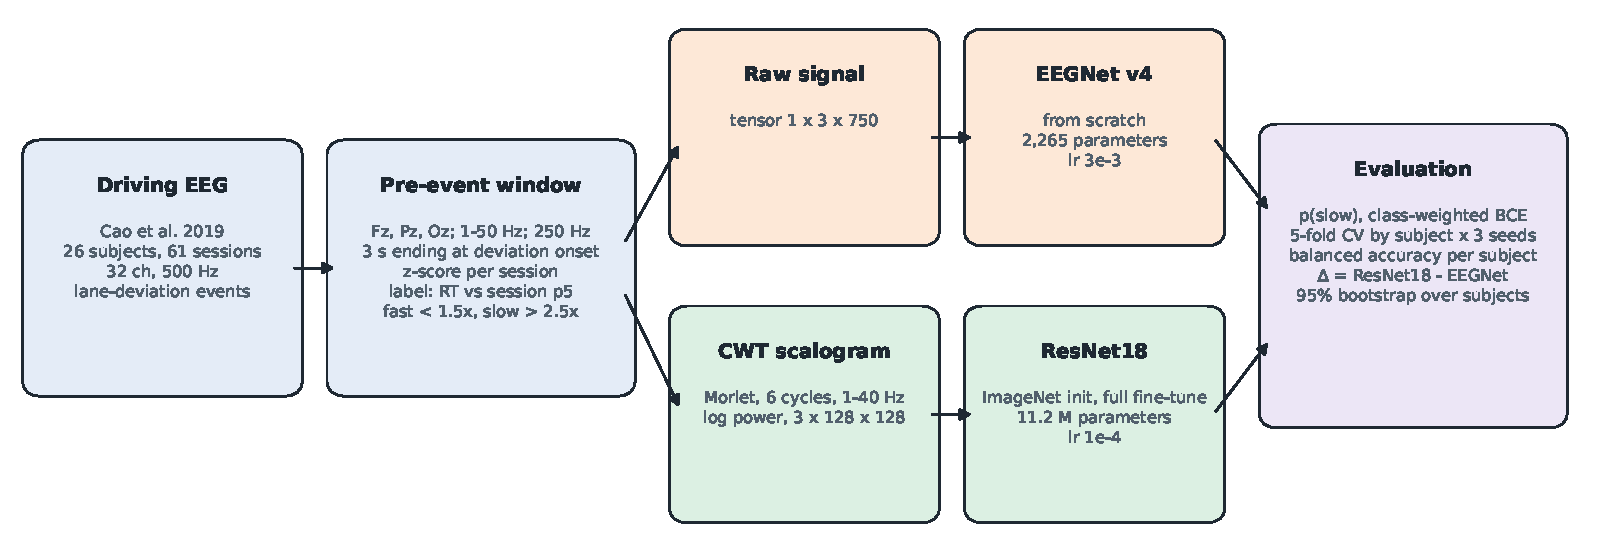
\includegraphics[width=0.95\textwidth]{pipeline}

\small
Cao et al.\ 2019: 26 subjects, 61 sessions, \textbf{18{,}087 windows} (27.6\% slow). Duplicate session removed (EEG sample-identical).
\end{frame}

\begin{frame}{Models and objective}
\small
\begin{tabular}{@{}lllll@{}}
\toprule
Role & Model & Input & Params & Training \\
\midrule
Main & ResNet18, ImageNet, full fine-tune & CWT $3\times128\times128$ & 11.2\,M & AdamW lr $3\!\times\!10^{-4}$, batch 64 \\
Baseline & EEGNet v4, from scratch & raw $1\times3\times750$ & 2{,}265 & AdamW lr $3\!\times\!10^{-3}$, batch 128 \\
Classical & Logistic reg.\ on log band power & 9 features & 10 & class-balanced \\
Controls & trial position; shuffled labels & & & \\
\bottomrule
\end{tabular}

\bigskip
\begin{itemize}
\item \textbf{Loss:} class-weighted binary cross-entropy on the slow logit
\item Same cap (80 epochs), patience 8, early stopping on 4 held-out \emph{training} subjects
\item \textbf{Matched tuning:} learning rate chosen on validation AUROC only (seed 0); CNN grid widened when its best rate sat at the edge
\end{itemize}
\end{frame}

% ~1 min
\begin{frame}{Experimental protocol}
\begin{itemize}
\item \textbf{5-fold CV by subject} $\times$ 3 seeds = 15 trainings per model; identical folds for all models
\item \textbf{Primary metric:} balanced accuracy per subject (24 subjects with $\geq$30 windows per class)
\item \textbf{Secondary:} AUROC. \textbf{Diagnostics:} channel/band EEGNet, per condition, Grad-CAM
\item \textbf{Uncertainty:} paired subject bootstrap (2{,}000); permutation test for real chance (within-session shuffle and circular shift)
\item \textbf{Compute:} Apple M1 Pro (MPS, float32) for all main runs; RTX 3080 replication
\item Reproducible: \texttt{config.yaml}, \texttt{train.py all}, \texttt{evaluate.py}
\end{itemize}
\end{frame}

% ~2 min
\begin{frame}{Main result: the hypothesis is not supported}
\centering
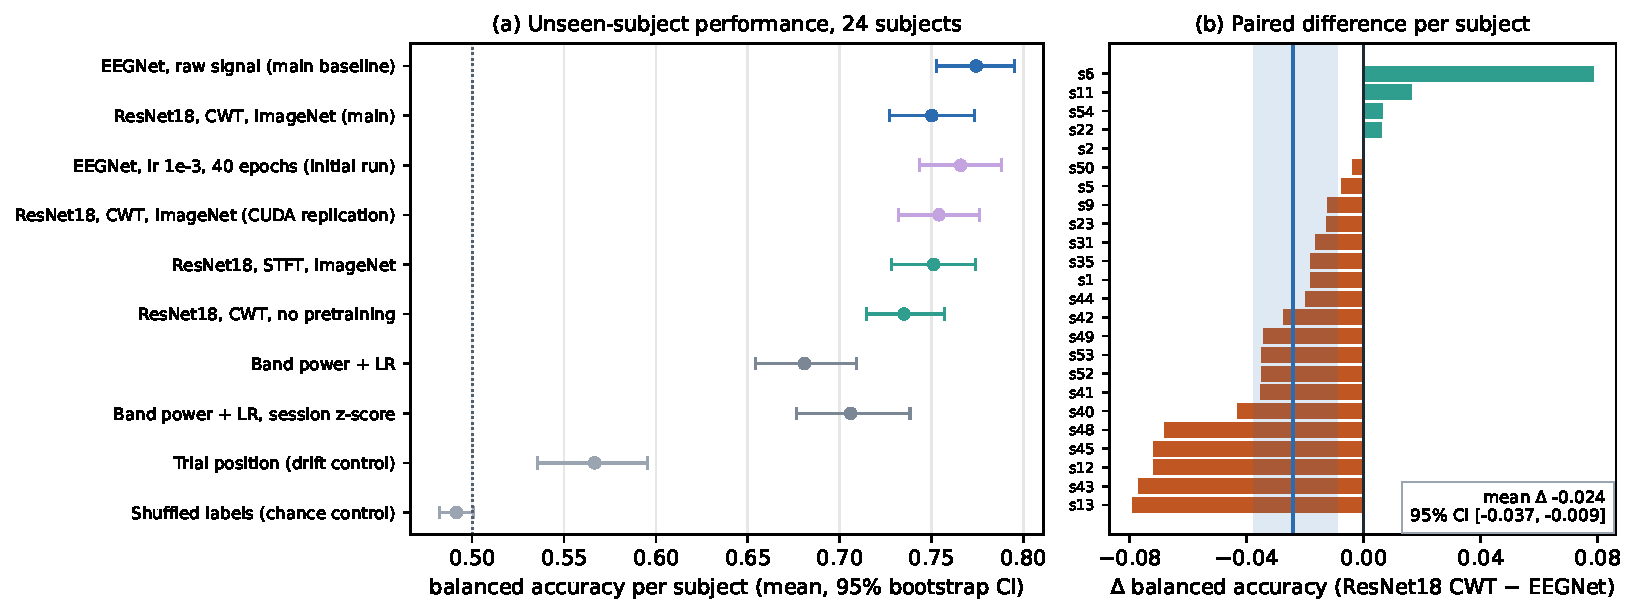
\includegraphics[width=0.92\textwidth]{fig_resultados}

\small
EEGNet \eegMainSubj{} vs.\ ResNet18 \resMainSubj{}. $\Delta=\deltaMain$, 95\% CI \ciMain{}: statistically a tie; ResNet18 better in \resBetter{} subjects.
\end{frame}

\begin{frame}{Is the result robust?}
\begin{itemize}
\item ResNet18 at the first grid's lr $10^{-4}$: $\Delta=\deltaOldLr$, CI \ciOldLr{} $\rightarrow$ ``EEGNet better'' was a tuning artifact; $3\!\times\!10^{-4}$ gains $\deltaLrGain$
\item Initial EEGNet (lr $10^{-3}$, 40 epochs): $\Delta=\deltaInitial$
\item CUDA replication of ResNet18: $\Delta=\deltaCuda$; CUDA vs.\ MPS differ by $\deltaCudaMps$ (CI \ciCudaMps)
\item Both networks $\gg$ band power (0.681), trial position (0.567), shuffled labels (0.491)
\item Permutation test: real per-subject chance $\approx$ 0.51--0.52; all networks $p<0.001$
\end{itemize}
\bigskip
\textbf{Reading:} a 2k-parameter network on the raw signal is at least as good as an 11M-parameter ImageNet CNN on images.
\end{frame}

% ~2 min
\begin{frame}{Ablations: one factor at a time}
\begin{columns}[T]
\column{0.5\textwidth}
\textbf{Pretraining} (same ResNet18, CWT, lr $10^{-4}$)
\begin{itemize}\small
\item ImageNet $-$ scratch: $\deltaScratch$, CI \ciScratch
\item Pretraining helps despite the domain gap
\end{itemize}
\medskip
\textbf{Representation} (CWT vs.\ STFT)
\begin{itemize}\small
\item CWT $-$ STFT: $\deltaStft$, CI \ciStft
\item Transform choice \stftShort
\end{itemize}
\column{0.5\textwidth}
\textbf{EEGNet: which signal carries the information?}
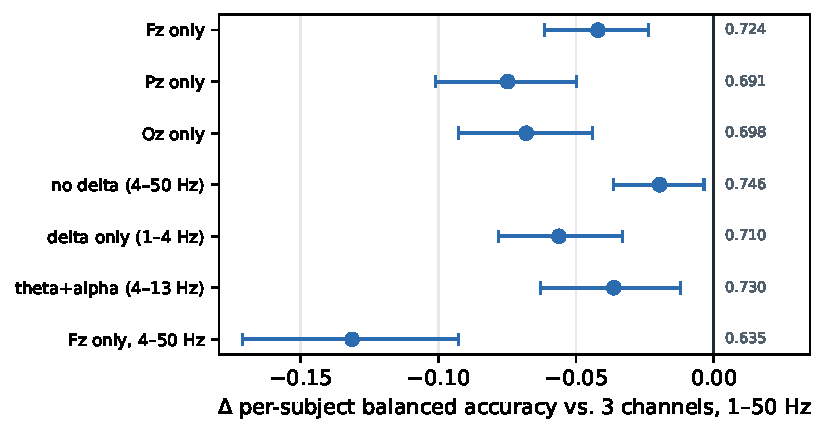
\includegraphics[width=\textwidth]{fig_diagnostico}
\end{columns}
\end{frame}

\begin{frame}{Qualitative diagnostic: what differs between classes?}
\centering
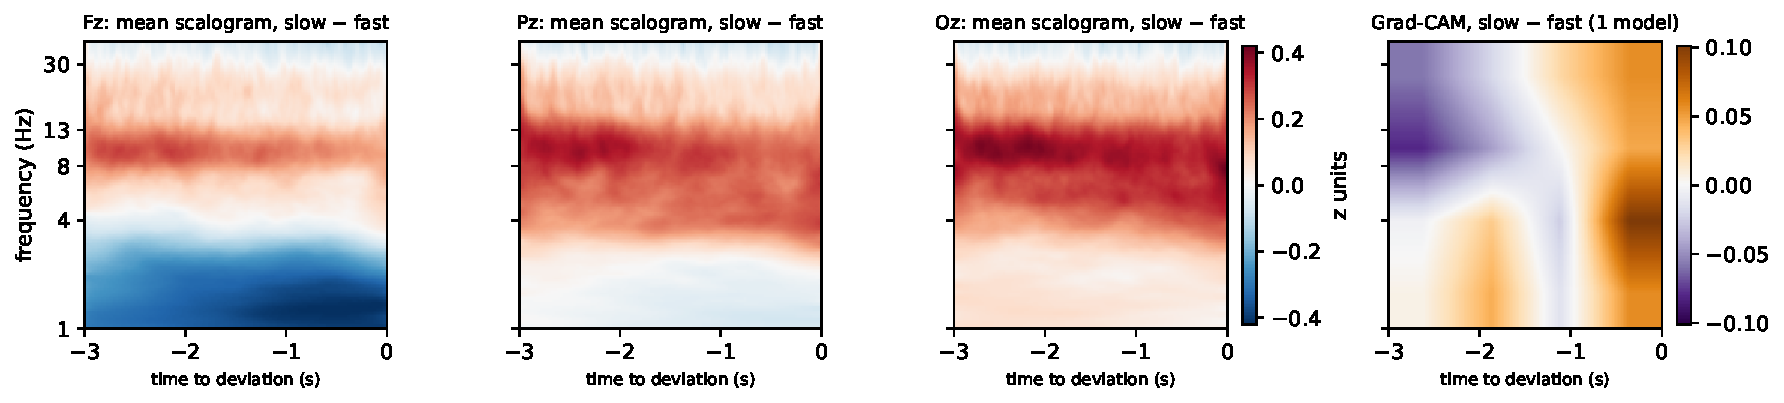
\includegraphics[width=\textwidth]{fig_interpretacion}

\begin{itemize}\small
\item Slow windows: more 4--13\,Hz power over the \emph{whole} 3\,s, strongest at Pz/Oz $\rightarrow$ looks like a state, not an event-locked response
\item Fz: less power below 4\,Hz in slow windows $\rightarrow$ possibly ocular, not cortical
\item Grad-CAM (right) is interpretation only, not evidence
\end{itemize}
\end{frame}

\begin{frame}{Failure analysis}
\begin{columns}[T]
\column{0.58\textwidth}
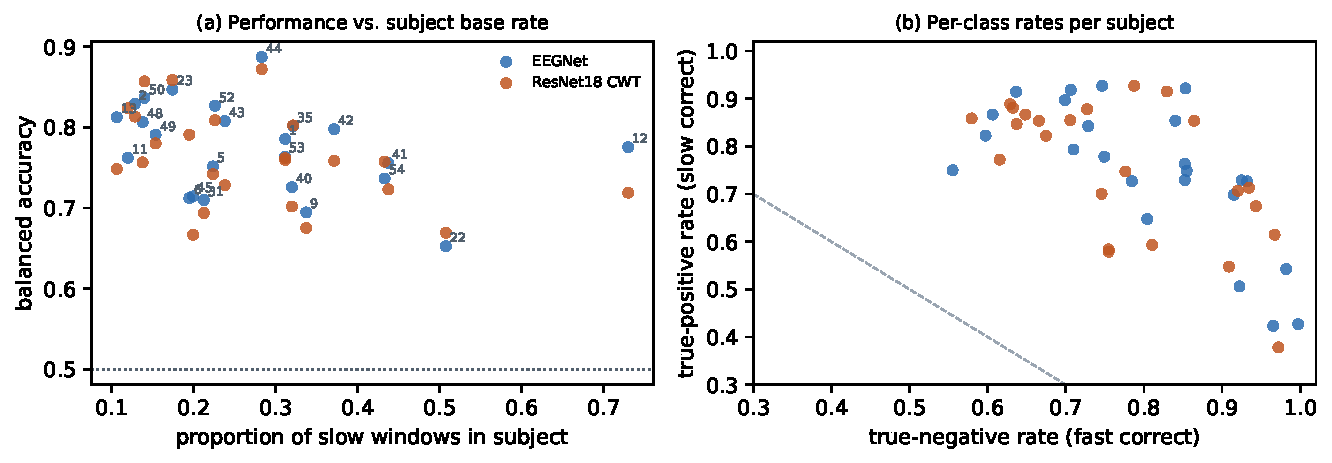
\includegraphics[width=\textwidth]{fig_fallos}
\column{0.42\textwidth}
\small
\begin{itemize}
\item Range \worstRange
\item Subjects with few slow trials: slow responses missed (high TNR, low TPR); subject 22 (51\% slow): the reverse $\rightarrow$ learned base rate
\item Models agree on \agreePct{} of windows; on disagreements \disagree
\item Both wrong: \bothWrongSlow{} slow (base 27.6\%)
\end{itemize}
\end{columns}
\end{frame}

\begin{frame}{Limitations}
\begin{itemize}
\item Labels are behavioral and session-relative, not a ground truth of drowsiness
\item Per-session z-score uses unlabeled test-session data (calibration period needed)
\item Slow trials cluster in time: windows not independent (we resample subjects)
\item ResNet18 peaks in 1--3 epochs and is lr-sensitive; schedules, augmentation, freezing not explored
\item EEGNet sometimes still improving at 80 epochs (gap can only widen)
\item One dataset, three channels: no claim about pain or trust yet
\end{itemize}
\end{frame}

% ~1 min
\begin{frame}{Conclusions and next thesis steps}
\textbf{Observed:} converting EEG to images does not improve cross-subject generalization here; EEGNet on the raw signal is at least as good. Pretraining helps the CNN; wavelet vs.\ STFT \stftShort.

\medskip
\textbf{Next steps}
\begin{itemize}
\item \textbf{Alberto:} apply the same protocol to the pain dataset (40 subjects) to predict subject-relative pain intensity; start from raw-signal EEGNet; repeat the channel/band diagnostic and add ICA/EOG control for ocular and muscle artifacts
\item \textbf{Juan Pablo:} apply the pipeline to the CARLA trust dataset (40 subjects)
\end{itemize}

\medskip
\centering\large Questions?
\end{frame}

\end{document}
